%-----------------------------------------------------------------
%	BASIC DOCUMENT LAYOUT
%-----------------------------------------------------------------
\documentclass[paper=a4, fontsize=12pt, twoside=semi, abstracton, listof=totoc, toc=left]{scrartcl}
\usepackage[T1]{fontenc}
\usepackage[utf8]{inputenc}
% \usepackage{lmodern}
\usepackage{newpxtext}
\usepackage{newpxmath}
\let\openbox\relax


\usepackage{caption}
\usepackage{subcaption}
\usepackage{pdfpages}

% \usepackage{kpfonts}
\usepackage{slantsc}
\usepackage{microtype}
\usepackage[british]{babel}
% \usepackage[backend=bibtex, style=phys, sorting=none, citestyle=authoryear, maxbibnames=3, maxcitenames=2]{biblatex}
\usepackage[backend=bibtex, style=trad-abbrv, sorting=none, maxbibnames=3, maxcitenames=2]{biblatex}
\addbibresource{bibliography.bib}
\makeatletter
	\def\blx@maxline{77}
\makeatother

% Sectioning layout
\addtokomafont{sectioning}{\normalfont\bfseries}
\usepackage{tocstyle}
\usetocstyle{standard}
\renewcommand*\descriptionlabel[1]{\hspace\labelsep\normalfont\bfseries{#1}}
\usepackage[titletoc]{appendix}

% Empty pages
\usepackage{etoolbox}
% \pretocmd{\toc}{\cleardoubleevenemptypage}{}{}
% \pretocmd{\section}{\cleardoubleevenemptypage}{}{}
\pretocmd{\part}{\cleardoubleevenemptypage\thispagestyle{empty}}{}{}
\renewcommand\partheadstartvskip{\clearpage\null\vfil}
\renewcommand\partheadmidvskip{\par\nobreak\vskip 20pt\thispagestyle{empty}}

% Paragraph indentation behaviour
\setlength{\parindent}{0pt}
\setlength{\parskip}{0.3\baselineskip plus2pt minus2pt}
\newcommand{\sk}{\medskip\noindent}

% Fancy header and footer
\usepackage{fancyhdr}
\pagestyle{fancyplain}
\fancyhead[LO]{\thepage}
\fancyhead[CO]{}
\fancyhead[RO]{\nouppercase{\mytitle}}
\fancyhead[LE]{\nouppercase{\rightmark}}
% \fancyhead[LE]{\nouppercase{\leftmark}}
\fancyhead[CE]{}
\fancyhead[RE]{\thepage}
\fancyfoot{}
\renewcommand{\headrulewidth}{0.3pt}
\renewcommand{\footrulewidth}{0pt}
\setlength{\headheight}{13.6pt}

%-----------------------------------------------------------------
%	MATHS AND SCIENCE
%-----------------------------------------------------------------
\usepackage{amsmath,amsfonts,amsthm,amssymb}
\usepackage{xfrac}
\usepackage[a]{esvect}
\usepackage{chemformula}
\usepackage{graphicx}
\usepackage{mathtools}

\usepackage[arrowdel]{physics}
	\renewcommand{\vnabla}{\vec{\nabla}}
	% \renewcommand{\vectorbold}[1]{\boldsymbol{#1}}
	% \renewcommand{\vectorarrow}[1]{\vec{\boldsymbol{#1}}}
	% \renewcommand{\vectorunit}[1]{\hat{\boldsymbol{#1}}}
	\renewcommand{\vectorarrow}[1]{\vec{#1}}
	\renewcommand{\vectorunit}[1]{\hat{#1}}
	\renewcommand*{\grad}[1]{\vnabla #1}
	\renewcommand*{\div}[1]{\vnabla \vdot \va{#1}}
	\renewcommand*{\curl}[1]{\vnabla \cp \va{#1}}
	\let\rot\curl

% SI units
\usepackage[separate-uncertainty=true]{siunitx}
% \sisetup{range-phrase = \text{--}, range-units = brackets}
\sisetup{range-phrase = \text{--}, range-units = single}
\DeclareSIPrePower\quartic{4}
	%\DeclareSIUnit\micron{\micro\metre}

% Smaller trig functions
\newcommand{\Sin}{\trigbraces{\operatorname{s}}}
\newcommand{\Cos}{\trigbraces{\operatorname{c}}}
\newcommand{\Tan}{\trigbraces{\operatorname{t}}}

% Operator-style notation for matrices
\newcommand*{\mat}[1]{\hat{#1}}

% Matrices in (A|B) form via [c|c] option
\makeatletter
\renewcommand*\env@matrix[1][*\c@MaxMatrixCols c]{%
  \hskip -\arraycolsep
  \let\@ifnextchar\new@ifnextchar
  \array{#1}}
\makeatother

% Shorter \mathcal and \mathbb
\newcommand*{\mc}[1]{\mathcal{#1}}
\newcommand*{\mbb}[1]{\mathbb{#1}}

% Shorter ^\ast and ^\dagger
\newcommand*{\sast}{^{\star}{}}
\newcommand*{\sdag}{^{\dagger}{}}

% Blackboard bold identity
\usepackage{bbm}
\newcommand*{\bbid}{\mathbbm{1}}

% Shorter displaystyle
\newcommand*{\dsp}{\displaystyle}

% Inexact differential
\newcommand{\dbar}{\mathchar'26\mkern-12mu\mathrm{d}}
\newcommand{\indd}[1]{\dbar{#1}}

% Arrows with text and cancels for developments
\newcommand{\tikzmark}[1]{\tikz[overlay,remember picture] \node (#1) {};}
\tikzset{square arrow/.style={to path={-- ++(0,-.25) -| (\tikztotarget)}}}
\usepackage{cancel}

\newcommand*\acr[1]{\textscale{.85}{#1}}

% Conditional Probability
\makeatletter
\newcommand{\@giventhatstar}[2]{\left(#1\;\middle|\;#2\right)}
\newcommand{\@giventhatnostar}[3][]{#1(#2\;#1|\;#3#1)}
\newcommand{\giventhat}{\@ifstar\@giventhatstar\@giventhatnostar}
\makeatother

% Expected Value
\DeclareMathOperator{\EX}{\mathbb{E}}% expected value


%-----------------------------------------------------------------
%   CODE
%------------------------------------------------------------------

\usepackage[linesnumbered,algoruled,vlined]{algorithm2e}
% \setlength{\algotitleheightrule}{0.8pt}
% \setlength{\algoheightrule}{0pt}

\makeatletter
\def\BState{\State\hskip-\ALG@thistlm}
\makeatother


%-----------------------------------------------------------------
%	OTHER PACKAGES
%-----------------------------------------------------------------
\usepackage{environ}

%Left numbered equations
\makeatletter
	\NewEnviron{Lalign}{\tagsleft@true\begin{align}\BODY\end{align}}
\makeatother

% Plots and graphics
\usepackage{pgfplots}
\usepackage{tikz}
\usepackage{color}
	\makeatletter
		\color{black}
		\let\default@color\current@color
	\makeatother

% Richer enumerate, figure, and table support
\usepackage{enumerate}
\usepackage[shortlabels]{enumitem}
\usepackage{float}
\usepackage{tabularx}
\usepackage{booktabs}
	%\setlength{\intextsep}{8pt}
% \numberwithin{equation}{section}
% \numberwithin{figure}{section}
% \numberwithin{table}{section}

% No indentation after certain environments
\makeatletter
\newcommand*\NoIndentAfterEnv[1]{%
	\AfterEndEnvironment{#1}{\par\@afterindentfalse\@afterheading}}
\makeatother
%\NoIndentAfterEnv{thm}
\NoIndentAfterEnv{defi}
\NoIndentAfterEnv{example}
\NoIndentAfterEnv{table}

% Misc packages
\usepackage{ccicons}
\usepackage{lipsum}
\usepackage{todonotes}
\usepackage{array}
\usepackage{multirow}

% Print DOI only if there's no URL
\renewbibmacro*{doi+eprint+url}{%
  \iftoggle{bbx:doi}
    {\iffieldundef{url}{\printfield{doi}}{}}
    {}%
  \newunit\newblock
  \iftoggle{bbx:eprint}
    {\usebibmacro{eprint}}
    {}%
  \newunit\newblock
  \iftoggle{bbx:url}
    {\usebibmacro{url+urldate}}
    {}}

%-----------------------------------------------------------------
%	PICANT PEDRA
%-----------------------------------------------------------------
\newcommand{\picpedra}[1]{%
\begin{tikzpicture}[#1, y=0.80pt,x=0.80pt,yscale=-1, inner sep=0pt, outer sep=0pt]
\begin{scope}[shift={(-138.30362,-166.74493)}]%
  \path[fill=black] (139.2176,188.4957) .. controls (138.9564,188.4159) and%
    (138.7011,188.2301) .. (138.5524,188.0114) .. controls (138.2978,187.6368) and%
    (138.2440,187.3211) .. (138.3663,186.9178) .. controls (138.4015,186.8018) and%
    (140.3831,183.4909) .. (142.7700,179.5601) -- (147.1098,172.4133) --%
    (146.9284,171.5442) -- (146.7470,170.6752) -- (145.7402,170.0523) .. controls%
    (143.4757,168.6512) and (142.8062,168.3226) .. (141.1474,167.7978) .. controls%
    (140.7529,167.6730) and (140.1861,167.5111) .. (139.8878,167.4381) --%
    (139.3454,167.3053) -- (139.3776,167.0906) .. controls (139.4212,166.7995) and%
    (139.4468,166.7447) .. (139.5388,166.7449) .. controls (139.7032,166.7454) and%
    (141.6511,166.9894) .. (142.2027,167.0786) .. controls (143.9483,167.3608) and%
    (145.3942,167.8733) .. (147.0970,168.8132) .. controls (148.2905,169.4720) and%
    (154.4206,173.2611) .. (154.3961,173.3249) .. controls (154.3786,173.3705) and%
    (152.7303,176.1152) .. (152.6683,176.2020) .. controls (152.6623,176.2100) and%
    (151.8971,175.7280) .. (150.9669,175.1314) .. controls (150.0368,174.5348) and%
    (149.2502,174.0443) .. (149.2189,174.0415) .. controls (149.1877,174.0385) and%
    (147.2495,177.1669) .. (144.9117,180.9932) .. controls (142.3326,185.2145) and%
    (140.5841,188.0293) .. (140.4650,188.1514) .. controls (140.3571,188.2621) and%
    (140.1876,188.3866) .. (140.0883,188.4281) .. controls (139.8565,188.5250) and%
    (139.4235,188.5586) .. (139.2176,188.4957) -- cycle(148.9649,187.8028) ..%
    controls (148.0576,187.4766) and (147.2700,187.1899) .. (147.2146,187.1657) ..%
    controls (147.1146,187.1220) and (147.1162,187.1114) .. (147.4146,185.8217) ..%
    controls (147.5800,185.1068) and (147.7222,184.5162) .. (147.7305,184.5092) ..%
    controls (147.7527,184.4907) and (150.6462,183.6346) .. (150.7516,183.6154) ..%
    controls (150.8304,183.6010) and (150.9165,183.8519) .. (151.4828,185.7466) ..%
    controls (151.8359,186.9278) and (152.1158,187.9176) .. (152.1048,187.9463) ..%
    controls (152.0862,187.9947) and (150.7675,188.4095) .. (150.6620,188.4001) ..%
    controls (150.6359,188.3981) and (149.8722,188.1290) .. (148.9649,187.8028) --%
    cycle(154.1766,185.9653) -- (154.1766,183.7654) -- (156.3402,183.7779) --%
    (158.5037,183.7904) -- (158.5160,185.2248) -- (158.5282,186.6593) --%
    (157.8302,187.4123) -- (157.1323,188.1654) -- (155.6544,188.1654) --%
    (154.1765,188.1654) -- (154.1765,185.9655) -- cycle(152.6388,182.7681) --%
    (152.0905,182.2958) -- (152.0024,181.2179) -- (151.9143,180.1401) --%
    (152.3828,179.5847) .. controls (152.6405,179.2793) and (152.8669,179.0356) ..%
    (152.8859,179.0431) .. controls (152.9939,179.0859) and (155.1259,180.9305) ..%
    (155.1182,180.9745) .. controls (155.1077,181.0344) and (153.2599,183.2318) ..%
    (153.2156,183.2370) .. controls (153.1999,183.2390) and (152.9403,183.0279) ..%
    (152.6387,182.7681) -- cycle;%
\end{scope}%
\end{tikzpicture}%
}

\newcommand*{\pedra}{\overset{\picpedra{scale=0.5}\,}{\cdots}}{}



%-----------------------------------------------------------------
%	SYNTAX HIGHLIGHTING
%-----------------------------------------------------------------
\usepackage[formats]{listings}
\usepackage{relsize}
\usepackage{chngcntr}

\renewcommand{\lstlistingname}{Snippet}
\renewcommand{\lstlistlistingname}{List of snippets}

\lstloadlanguages{R}
\lstdefinelanguage{Renhanced}[]{R}{%
	morekeywords={acf,ar,arima,arima.sim,colMeans,colSums,is.na,is.null,%
	mapply,ms,na.rm,nlmin,replicate,row.names,rowMeans,rowSums,seasonal,%
	sys.time,system.time,ts.plot,which.max,which.min,%
	rename,mutate,unite,select,filter,left_join,group_by,dplyr::select,%
	ggplot,aes,geom_line,geom_hline,geom_point,geom_path,geom_errorbar,%
	geom_abline,geom_smooth%
	geom_cartogram,coord_proj,scale_x_longitude, scale_y_latitude,%
	labs,guides,annotate,theme,rowwise,%
	scale_linetype_manual,scale_colour_manual,scale_x_log10,scale_y_log10,%
	attr,paste,paste0,bind_rows,str_trim,as.numeric,as.dataframe,data.frame},
	deletekeywords={c,range,step},
	alsoletter={.,_,::},
	otherkeywords = {!,!=,~,\$,*,\&,\%/\%,\%*\%,\%\%,\%>\%,<-,<<-,\% in \%}
	}

\newcommand*{\inline}{\lstinline[basicstyle=\normalsize\ttfamily]}


\lstset{language=C,
		frame=tb,
		% captionpos=b,
		tabsize=2,
		% showtabs=true,
		breaklines=true,
		breakatwhitespace=true,
		basicstyle=\smaller\ttfamily,
		numbers=left,
		numberstyle=\tiny,
		numbersep=7.5pt,
		% commentstyle=\textsl,
		xleftmargin=3ex}
\lstset{escapeinside={(*}{*)}}   % for (*\ref{ }*) inside lstlistings (Scode)

\usepackage{xcolor}
\newcommand\crule[3][black]{\textcolor{#1}{\rule{#2}{#3}}}
\definecolor{mypurple}{RGB}{147, 34, 156}
\definecolor{mypink}{RGB}{255, 0, 110}
\definecolor{myblue}{RGB}{69, 57, 252}
\definecolor{myorange}{RGB}{246, 149, 50}
\definecolor{mygreen}{RGB}{73, 166, 87}

%-----------------------------------------------------------------
%	THEOREMS
%-----------------------------------------------------------------
\usepackage{thmtools}

% Theroems layout
\declaretheoremstyle[
	spaceabove=6pt, spacebelow=6pt,
	headfont=\normalfont,
	notefont=\mdseries, notebraces={(}{)},
	bodyfont=\small,
	postheadspace=1em,
]{small}

\declaretheorem[style=plain,name=Theorem,qed=$\square$,numberwithin=section]{thm}
\declaretheorem[style=plain,name=Corollary,qed=$\square$,sibling=thm]{cor}
\declaretheorem[style=plain,name=Lemma,qed=$\square$,sibling=thm]{lem}
\declaretheorem[style=definition,name=Definition,qed=$\blacksquare$,numberwithin=section]{defi}
\declaretheorem[style=definition,name=Example,qed=$\blacktriangle$,numberwithin=section]{example}
\declaretheorem[style=small,name=Proof,numbered=no,qed=$\square$]{sproof}

%-----------------------------------------------------------------
%	ELA MOTHERFUCKING GEMINADA
%-----------------------------------------------------------------
\def\xgem{%
	\ifmmode
		\csname normal@char\string"\endcsname l%
	\else
		\leftllkern=0pt\rightllkern=0pt\raiselldim=0pt
		\setbox0\hbox{l}\setbox1\hbox{l\/}\setbox2\hbox{.}%
		\advance\raiselldim by \the\fontdimen5\the\font
		\advance\raiselldim by -\ht2
		\leftllkern=-.25\wd0%
		\advance\leftllkern by \wd1
		\advance\leftllkern by -\wd0
		\rightllkern=-.25\wd0%
		\advance\rightllkern by -\wd1
		\advance\rightllkern by \wd0
		\allowhyphens\discretionary{-}{}%
		{\kern\leftllkern\raise\raiselldim\hbox{.}%
			\kern\rightllkern}\allowhyphens
	\fi
}
\def\Xgem{%
	\ifmmode
		\csname normal@char\string"\endcsname L%
	\else
		\leftllkern=0pt\rightllkern=0pt\raiselldim=0pt
		\setbox0\hbox{L}\setbox1\hbox{L\/}\setbox2\hbox{.}%
		\advance\raiselldim by .5\ht0
		\advance\raiselldim by -.5\ht2
		\leftllkern=-.125\wd0%
		\advance\leftllkern by \wd1
		\advance\leftllkern by -\wd0
		\rightllkern=-\wd0%
		\divide\rightllkern by 6
		\advance\rightllkern by -\wd1
		\advance\rightllkern by \wd0
		\allowhyphens\discretionary{-}{}%
		{\kern\leftllkern\raise\raiselldim\hbox{.}%
			\kern\rightllkern}\allowhyphens
	\fi
}

\expandafter\let\expandafter\saveperiodcentered
	\csname T1\string\textperiodcentered \endcsname

\DeclareTextCommand{\textperiodcentered}{T1}[1]{%
	\ifnum\spacefactor=998
		\Xgem
	\else
		\xgem
	\fi#1}

%-----------------------------------------------------------------
%	DEDICATION ENVIRONMENT
%-----------------------------------------------------------------

\newenvironment{mydedication}
	{\clearpage           % we want a new page
	\thispagestyle{empty}% no header and footer
	\vspace*{\stretch{1}}% some space at the top
	\itshape             % the text is in italics
	\raggedleft          % flush to the right margin
	}
	{\par % end the paragraph
	\vspace{\stretch{3}} % space at bottom is three times that at the top
	\clearpage           % finish off the page
	}

%-----------------------------------------------------------------
%	PDF INFO AND HYPERREF
%-----------------------------------------------------------------
\usepackage{hyperref}
\hypersetup{colorlinks, citecolor=black, filecolor=black, linkcolor=black, urlcolor=black}
\usepackage{cleveref}
	\crefname{section}{\S}{\SS}
	\Crefname{section}{\S}{\SS}
	\crefname{listing}{snippet}{}

\newcommand*{\mytitle}{On Savings Optimisation Strategies}
\newcommand*{\mysubtitle}{Pooled Funds and scale-free and location-free risk measures}
\newcommand*{\myauthor}{Alejandro Jiménez Rico}
\newcommand*{\mysupervisor}{Isabel Serra \& Montserrat Guillén}
\newcommand*{\mytutor}{Isabel Serra}
\newcommand*{\myuni}{Centre de Recerca  Matemàtica}
\newcommand*{\mydate}{2018}

\pdfstringdefDisableCommands{\def\and{and }}

\usepackage{hyperxmp}
\hypersetup{pdfauthor={\myauthor}, pdftitle={\mytitle}}

%-----------------------------------------------------------------
%	TITLE SECTION AND DOCUMENT BEGINNING
%-----------------------------------------------------------------
\newcommand{\horrule}[1]{\rule{\linewidth}{#1}}
\title{
	\normalfont
	\small \scshape{\myuni} \\ [25pt]
	\horrule{0.5pt} \\ [0.4cm]
	\Huge \mytitle \\[0.2cm]
	% \large \mysubtitle \\
	\horrule{2pt} \\ [10.5cm]
}

\author{
	\myauthor \\
	\small Academic tutor: \mytutor \\
	\small Supervised by: \mysupervisor
}

\date{\mydate}

\begin{document}


\includepdf[pages={-1}]{cover.pdf}
\newpage
%\counterwithin{lstlisting}{section}

\clearpage
\maketitle
\thispagestyle{empty}
\addtocounter{page}{-1}

%-----------------------------------------------------------------
%	DEDICATION
%-----------------------------------------------------------------
\begin{mydedication}
	A man got to have a code. \\[0.1cm]
	\emph{Omar Little}
\end{mydedication}

% ---------------------------------------------------------
%   QUOTES
%----------------------------------------------------------



%-----------------------------------------------------------------
%	DOCUMENT BODY
%-----------------------------------------------------------------
% \cleardoubleevenemptypage
\cleardoubleevenemptypage
\thispagestyle{empty}
\phantomsection
\addcontentsline{toc}{section}{Abstract}
\begin{abstract}

In classical savings theory it is stated that the optimal way to ensure a risk level is to set a constant proportion of risky assets at all time. This way, most savings strategies try to optimize their results based on a fixed risk aversion profile initially settled by the investor. Usually, funds arranging pension plans manage their fund as the result of the sum of many individually isolated investors, with no consideration upon the opportunities present in more collectively-managed schemes.

Throughout this work we will replicate the results of an alternative optimal strategy that changes proportion invested in risky assets along time, instead of setting an initial constan proportion; and we will confirm that this kind of strategy does not impede to set a fixed risk aversion profile. Moreover, we will incorporate the concept of Pooled Funds to those schemes and compare their performances using standard risk measures.

Finally, we will study the risk profile of all previously developed strategies on the article using Tail Distribution Modelling and Extreme Value Analysis in order to contrast the particularities of location and scale free risk measures.

\end{abstract}


\pdfbookmark[1]{\contentsname}{toc}
\tableofcontents

%-----------------------------------------------------------------
%	INTRODUCTION
%	!TEX root = ./../main.tex
%-----------------------------------------------------------------
\section{Introduction}

The reason for saving is to utilise the present wealth of a saver in order to build a retirement plan that secures a safe stream of capital for when it may be needed. This future condition need can be thought as deterministic, as we usually think in a typical pension plan, when there is a fixed time scheme when the saver starts collecting his money and when it ends; or it can be subject to some non-deterministic eventuality, as in most insurance plans. This kind of investment is, thus, characterised by an initial period in which the investor is saving money followed by a period of consumption, once the investor satisfies that future condition.

Hence, every savings strategy should aim at maximising that final capital whilst \textit{securing} it. In general, we could say that there is a trade-off between that maximisation of capital (return) and the degree of its security (risk). The balance between these two magnitudes is what savings strategies try to optimise.

It is obvious that every saver would like to maximise the return of his money. But if we accept that this can only be accomplished at the expense of more risk, the investor has to decide which degree of risk is she able to tolerate, setting a risk limit. This decision upon the exposure to risk is what defines the \textit{risk aversion} profile of every investor.

Most savings strategies are measured setting a fixed risk limit provided by a risk aversion profile, thus maximising the returns that can be extracted once that risk limit is provided. Thus, the great interest canalized on testing and analysing the results of different savings strategies using the return and the risk as measures of performance.

% Throughout this work, we will make use of the risk adjusted ad hoc performance measure, recently developed in~\cite{a:guillen-performance, a:guillen-guarantee}, in order to evaluate our models.

Throughout this project we will compare the results obtained from many different savings strategies, and we will compare their risk and return. The set up for all of them will be the same. A simulated investor will save up a yearly fixed amount of money from the age of 30 years and, after that, she will consume the same amount for the next 30 years. Part of the saved money will be invested in risky assets whilst the rest will be invested in risk-free assets. The main question to be addressed is going to be the optimal proportion of the investment exposed to risky assets, and whether the fund is managing the investors isolated or collectively.

Firstly, we will study the results obtained from~\cite{a:guillen-optimisation} and compare the two strategies involved in their study: The benchmark and what we call the \emph{Alternative} strategy.

In the case that we use as a benchmark, called \textit{Constant Proportion Portfolio Insurance} (CPPI), introduced by \cite{a:perold-constant}, a constant proportion of the wealth to be invested is allocated in risky assets, whereas the rest is allocated in non-risky assets. This means that the same proportion of the investment will be invested in the risky market, year over year.

The Alternative scheme, developed in \cite{a:guillen-optimisation}, consists of a different approach regarding that proportion of risky investment. Instead of a time-constant proportion, this model suggests a variable proportion that follows a formula that takes into account the present wealth of the investor. We will explain this formula in the following chapters.

Later on, we will include the concept of a \emph{Pooled Fund}, in which the savers are not considered in isolation, but parts of a whole Fund. The main characteristic of considering the saver within a common Pooled Fund is the concept of mortality. There is always a risk that the saver does not live up to retire and collect back the fruit of her savings. Taking that risk into account, we will show how the wealth of those unlucky deceased investors can be distributed among the survivors. Moreover, we will test both previously described strategies in the context of a Pooled Fund and analyse their performance.

Throughout the majority of this work, we will make use of the risk adjusted ad hoc performance measure, recently developed in~\cite{a:guillen-performance, a:guillen-guarantee}, in order to evaluate our models. Yet in the final section we will develop and explain some other measures of Risk that are more sensible to worst-case scenarios and larger losses, becoming another useful tool to assess risk and performance of Investment and Savings Strategies.

\section{Background On Risk Measures} \label{sec:risk}

When simulating a savings scheme, the first assumption is regarding risk. It is usual to make a stark distinction between risky and risk-free investments.

But what do we mean by \textit{risk}? It is common to define risk as the uncertainty of the outcome of a given investment. So if we save some money at a $0.1 \%$ bank deposit, we can fairly assume that this investment is risk-free, because we know how much money we will receive at the end. A different scenario could be to invest this money in some market-dependent asset with $1 \%$ expected return but no guarantee of that return.

But how do we reckon that degree of uncertainty? In stock markets is usual to assume that the price of stocks behaviour is a brownian motion (see~\cite{b:cootner-random, a:samuelson-speculative}), and as such we can define their movement by \textit{trend} and \textit{dispersion} parameters. Since the return obtained by investing in stock assets comes from the relative difference in price between purchase and selling, it is easy to deduce that if we assume that the price follows a geometric brownian motion with trend $\mu$ and dispersion $\sigma$, the expected return of our investment would be $\mu$ with standard deviation $\sigma$. Thanks to this mathematical scheme, we can numerically define the expected return and some degree of uncertainty on it that we will henceforth use as our starting theoretical point. So, the returns at time $t$ are defined as:

\begin{align} \label{eq:return}
    R_t = \frac{P_t - P_{t-1}}{P_{t-1}}\textit{.}
\end{align}

Where $P_t$ is the price of a stock at time $t$ and $P_{t-1}$ is the price of the stock at time $t-1$.

Even though many different models can be assumed to describe the behaviour of financial markets, the point of this section is to understand and exemplify the set up necessary in order to decide how we measure risk.

Using the standard definition of risk, any unexpected uplift from the expected return would be considered under the umbrella of 'risky outcomes'. Since it is kind of counter-intuitive to assume the probability of a positive outcome as 'risk'. Another way to look at the risk definition is not just looking at dispersion, but one half of that dispersion. Thus, is not unreasonable to assume as risk just the negative part of the distribution of the random variable\footnote{Losses are settled negative and profits are positive.}.

\begin{figure}
    \centering
    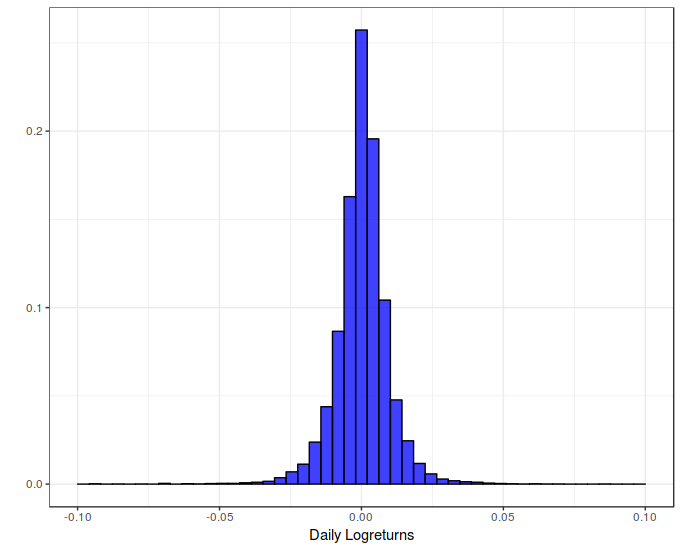
\includegraphics[scale=0.65]{./images/sp_hist.png}
    \caption{Daily logreturns of the Standard \& Poors index [1950 - 2017]. Data from Yahoo Finance.}
    \label{fig:daily-logreturns-sp}
\end{figure}

If we take a look at the actual observed returns in the stock market - as shown in figure~\ref{fig:daily-logreturns-sp} we can see the frequency of different returns. With a bit of imagination, we can notice a \textit{Bell Curve} shape, and so we could  think of a normal distribution of the logreturns. Where \textit{logreturns} are defined as:

\begin{align} \label{eq:logreturn}
    r_t = \ln{(1+R_t)}\textit{.}
\end{align}

This bell-shaped distribution is important because many financial models assume normality; see Modern Portfolio Theory~\cite{a:markowitz-portfolio}, efficient markets and the Black-Scholes option pricing model. And it is this very normality one of the main assumptions of the geometric brownian motion hypothesis of prices.

But given the irrational and unpredictable behaviour of the markets, we can see some flaws to this normality. Like the fat tails on the extremes of that histogram, fatter than they should, given normality. This little deviation implies that improbable events happen \textit{a lot} more than expected, and this rises a philosophical doubt that undermines our understanding of risk. A normal distribution assumes that, given enough observations, all values in the sample will be distributed equally above and below the mean. Hence, the convenience of using standard deviation as a measure of volatility, since it gives us some sense of how far away we can be from the mean. However, given the size of those extreme values, we can not entirely rely our assessment of risk upon the standard deviation; and thus we ought to study and gauge those fat tails further.

\subsection*{Expected Shortfall}

In order to measure the importance and the impact of the tails of return distributions, it is common to compute what is called the \textit{Expected Shortfall}. The Expected Shortfall ($ES_{\alpha}$) at an $\alpha$ quantile of a given distribution $X$ is defined~\cite{a:mcneil-es} as:

\begin{align} \label{expected-shortfall}
ES_{\alpha} = \frac{1}{\alpha}\int_{0}^{\alpha}VaR_{\gamma}\qty(X)d\gamma \textit{,}
\end{align}

Where $\alpha \in \qty(0,1)$, $VaR_{\gamma}\qty(X)$ is the $1-\gamma$ quantile of $X$ and $\gamma \in \qty(0,1)$. This means that the $ES_{\alpha}$ gives us the expected value of the returns distribution in the worst $\alpha \%$ cases. Which, in case of a continuous $X$, can be expressed as

\begin{align}
	ES_{\alpha} = \EX\giventhat{X}{X < VaR(X)}\emph{.}
\end{align}

Thus, the Expected Shortfall gives us a much more intuitive and reliable sense of the \textit{risk} of any investment; in addition to its useful mathematical properties~\cite{a:bertsimas-shortfall}.


\section{CPPI}

Firstly, we will start explainning what will be the \textit{benchmark} model. The constant portfolio strategy follows the logic derived from constant relative risk exposure.

This methodology consists in investing a constant proportion $\pi$ of the savings in risky assets (subject to volatility), whilst invetsing the rest $1 - \pi$ in risk-free assets. The point of this strategy is to present an intuitive straightforward way to control the risk exposure in savings strategies. The simplicity of this approach let us tweak $\pi$ in order to make the investment best suited for the risk aversion profile of each investor individually.

\subsection*{Simulation}

In order to simulate the performance of this kind of strategy, we start assuming that the risky assets follow a simplified geometric brownian motion, with \emph{trend} $\alpha$ and \emph{volatility} $\sigma$. Thus, if the saver invests $x$ in this asset at day $t$, the wealth of the saver at the next day would be $x_{t+1} = (1 + N\qty(\alpha, \sigma)) x_t$.

This way, we construct the scenario of an investor, saving a fixed amount of money $a$  trhoughout $T/2$ years, and that money being allocated $( 1 - \pi) a$ in the risk-free asset, whose value would be constant; and $\pi a$ allocated in the risky asset. Thus, if we set $x_t$ as the wealth at any given time $t$, we can see that

\begin{align}
	x_{t+1} = (1+N(\alpha, \sigma))x_{t}\pi + (1 - \pi)x_{t} + a
\end{align}

At some point in time, our investor will saving money and will start consuming it (as in most pension plans), so we just convert that fixed amount of money $a$ to \emph{consumed} money instead of saved. Thus, the evolution of wealth turns to be

\begin{align}
	x_{t+1} = x_{t}(1+N(\alpha, \sigma))\pi + (1 - \pi)x_{t} - a
\end{align}

At the end of all $T$ years, the final wealth $X_T$ reamining to the saver it is stored, and then all the process is repeated. This way we manage to compute tens of thousands of different performances and make some statistics out of them.


\subsection{Alternative Scheme}

Now that the CPPI model is presented and its logic understood, we can move upon to alternatives. One of the main characteristics of the CPPI model is that it is defined thanks to a constant, invariant $\pi$ that settles the risk exposure of the investor. An interesting approach would not just change this parameter, but make it \emph{variable}.

Normally, the simplest approach to ensure that an investment has a defined and controlled risk profile is to set a $\pi$ constant proportion of the investment to be allocated in risky assets, as done in the CPPI. That proportion is defined by the risk aversion profile of the investor, but is invariable throughout the investment.

However, the work of \cite{a:guillen-optimisation} showed that, given some investment plan ending at time $T$ with $X(T)$ final wealth, risk aversion profile defined by $\gamma$ and a maximum possible allowed loss $K$, we can set the utility function

\begin{align}
    u_\gamma = \frac{1}{\gamma}\qty(X(T) + K)^\gamma \emph{.}
\end{align}

Whose expected value for any given present wealth $x = X(t)$ is defined as

\begin{align}\label{eq:maxE}
    \max_{\pi}\EX\giventhat{u_{X(T)}}{x} \emph{,}
\end{align}

which can be maximized~\cite{a:guillen-optimisation} by a strategy that invests a relative amount in risky assets variable at any time $t \in [0,T)$, whose solution is:

\begin{align}\label{eq:the_formula}
    \pi(t)X(t) = A\qty(K + X(t) + g(t)) \textit{.}
\end{align}

Where $X(t)$ is the wealth at time $t$, $A$ is a parameter that defines the risk aversion profile of the investor, $K$ is the maximum loss the investor is capable to handle and $g(t)$ is the sum of all remaining inputs or outputs of money~\footnote{In \cite{a:donnelly-savings-decisions}'s work, the authors defined optimal savings strategies and analysed different updating periods for $\pi$.}: $g(t) = \sum_{i=t}^{T}a_i$. Thus, the time evolution of the wealth $X$ of an investor would behave as following:

\begin{align}
    dX = \alpha \pi(t)X(t)dt + \sigma \pi(t)X(t)dW(t) + dC(t)\textit{.}
\end{align}

Where $\alpha$ is the expected return of the risky market, $\sigma$ is the expected volatility of the risky market, $W(t)$ is a Wiener process and $C(t)$ is the allocated or consumed capital by the investor at every time step.

\subsection*{Simulation}

In order to analyse the alternative scheme, the process will be quite similar to the previous one. We set the normal behaviour of the price evolution of the risky asset, and fix all parameters. Thus, the wealth of the investor behaves as follows:

\begin{align}
    X_{t+1} = \qty(1+N(\alpha, \sigma))X_t \pi_t + \qty(1 - \pi_t)X_t + C(t) \textit{,}
\end{align}

where

\begin{align}
    \pi_t = \frac{A\qty(K + X_T + \sum_t^T C(t))}{X_T} \quad \textit{and}
\end{align}

\begin{equation*}
    C(t) =
    \begin{cases*}
      a & if $t <= T/2$ \\
      -a       & if $t > T/2$ \textit{.}
    \end{cases*}
\end{equation*}

Again, at the end of all $T$ years, the final wealth $X_T$ remaining to the saver it is stored, and then all the process is repeated. This way we manage to compute tens of thousands of different performances and make some statistics out of them.

\begin{figure}[H]
    \centering
    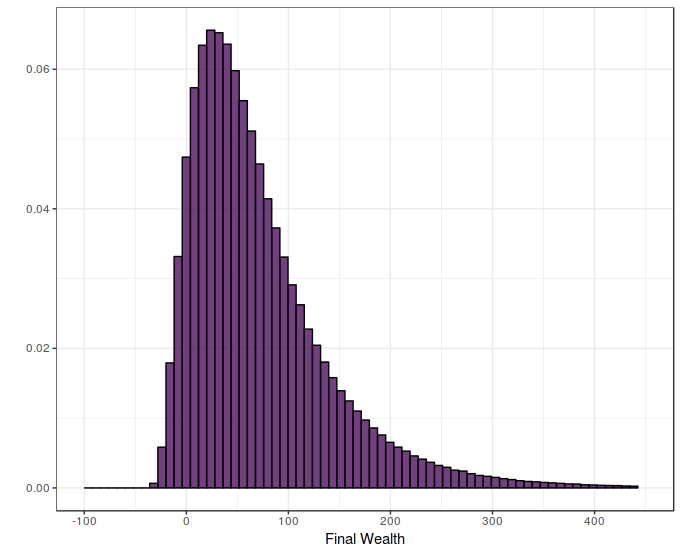
\includegraphics[scale=0.65]{./images/fw_alt.png}
    \caption{Results of $100,000$ simulations for the \textit{Alternative} model. Final wealth obtained for every simulation, where $T=30$, $\mu = 0.0343$, $\sigma = 0.1544$, $a=10$, $\pi = 0.1$.}
    \label{fig:alt_fw}
\end{figure}

In the case of figure \ref{fig:alt_fw}, where the right tail corresponds to large values of wealth, whereas the left part deals with losses; we can see how outrageously obvious is that it does \textit{not} follow a Normal Distribution.

The code necessary to replicate these results in R can be found in Appendix \ref{ap:alt-simple}.

\subsection{Comparison}

At this moment, we have understood and tested both strategies, and it is moment to contrast each other and highlight their differences.

First of all we plot together the frequency histograms for the final wealth distribution for both models.

\begin{figure}[H]
    \centering
    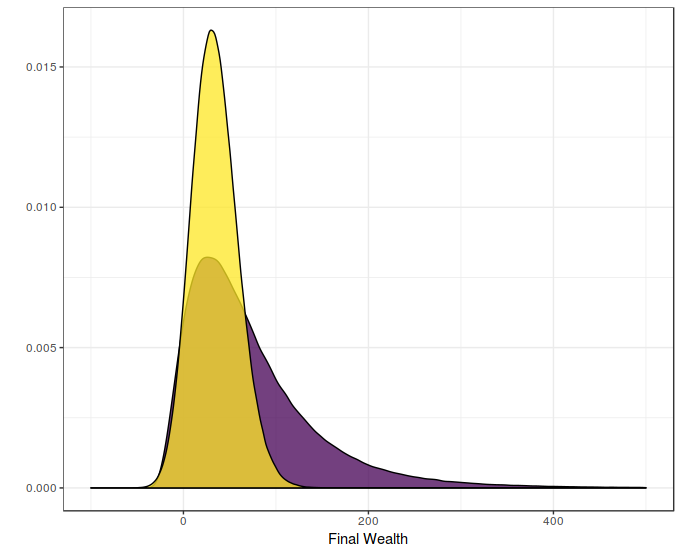
\includegraphics[scale=0.65]{./images/fw_both.png}
    \caption{Results of the simulation for the both models. Final wealth obtained for every simulation. The yellow one is the CPPI, and the purple one is the Alternative.}
    \label{fig:both_fw}
\end{figure}

Looking at Figure \ref{fig:both_fw} we may notice that they follow a considerably different distribution. We could say that the alternative model presents more dispersion, even though it is always a \textit{positive} deviation from the mean. 

In section \ref{sec:risk} we have discussed a little bit some implications of the definition of risk. Affirm that the alternative model presents more risk, just because its result is more disperse, would may seem a little simplistic. 

On the other hand, we can take a look at those rare cases when the final wealth happens to be negative. These are the cases worth exploring, for it is the scenario every investor is afraid of: losing money. Zooming in into the negative zone, as shown in figure \ref{fig:loss_both}, we can focus in the difference between the two models. Even though we can see some spurious differences in some places, the most honest answer is that it is not clear whose result is less risky.

\begin{figure}[H]
    \centering
    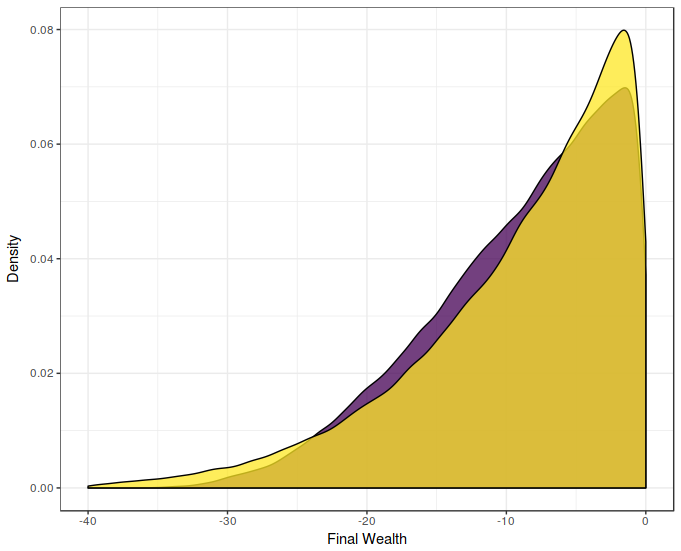
\includegraphics[scale=0.5]{./images/loss_both.png}
    \caption{Results of the simulation for the both models. Final wealth, filtered by negative values obtained for every simulation. The yellow one is the CPPI, and the purple one is the Alternative.}
    \label{fig:loss_both}
\end{figure}

In order to compare the degree of risk taken by every model, we make use of the \textit{Expected Shortfall}, as explained in section \ref{sec:risk}. If we set this parameter as the level of risk and we set it constant in both models, we can compare their returns. In~\cite{a:guillen-optimisation} it is shown that the Alternative model is able to set its Expected Shortfall (ES) by its $K$, using a closed formula.

Therefore, the approach is the following: We set a constant proportion $\pi$ for the CPPI model, we simulate it many times and measure the ES for the results. Then we find the $K$ in order to set the same ES on the Alternative model. This way we can simulate both models making sure they will assume the same risk, and thus we can freely compare their returns.

Setting $\alpha = 0.343$, $\sigma = 0.1544$, $a = 10$, $T = 60$, $A = 0.5$ and number of simulations $N = 100,000$ we find the results shown in table \ref{tab:cppi_alt}, in which we can see the outperformance of the alternative model, for many different levels of risk.

\begin{table}[H]
\centering
\caption{Results of $100,000$ simulations using different risk levels. These results match approximately those presented in \cite{a:guillen-optimisation}, on Table 1 at page 8. Any differences are attributable to the intrinsic randomness of simulations.}
\label{tab:cppi_alt}
\begin{tabular}{ccccccc}
\textbf{$\pi$} & \textbf{ES } & \textbf{$K$} & \textbf{CPPI ret} & \textbf{Alt ret} & \textbf{diff}  & \textbf{equiv $\pi$}\\
0.1   & -12.47  & 40.59  & 0.33     & 0.51    & 0.18    & 0.17\\
0.2   & -27.03  & 87.98  & 0.65     & 0.98    & 0.38    & 0.30 \\
0.3   & -42.99  & 139.95 & 0.95     & 1.42    & 0.46    & 0.45 \\
0.4   & -60.13  & 195.71 & 1.23     & 1.83    & 0.60    & 0.61 \\
0.5   & -78.25  & 255.02 & 1.5      & 2.22    & 0.71    & 0.69 \\
0.6   & -99.96  & 325.36 & 1.76     & 2.63    & 0.87    & 0.92 \\
0.7   & -120.61 & 392.56 & 2.00     & 3.00    & 1.00    & * \\
0.8   & -144.71 & 471.02 & 2.23     & 3.40    & 1.17    & * \\
0.9   & -172.94 & 562.92 & 2.39     & 3.81    & 1.42    & * \\
1     & -205.09 & 667.57 & 2.58     & 4.27    & 1.70    & *
\end{tabular}
\end{table}

\section{Optimisation of Pooled Funds Investment Strategies}

So far, we have managed to test two different strategies. We have analysed their return and risk in a simulated scenario, within the context of a pension plan. In order to assess the risk of the strategies, so far we have been measuring the market risk of the investment, by computing the \emph{Expected Shortfall}. However, in real-scenario pension plans, there are plenty of other risks that should be taken into consideration. One important risk, not rarely underestimated, is the so-called \textbf{Longevity Risk}. Longevity risk is referred to the probability of retirees that will live longer than expected and will thus exhaust all their savings. This possibility might doom some individuals to utter poverty or to burden relatives if the pension provider is not responsible for this kind of risk and all the costs incurred.

Recently, two worldwide phenomena ought to be highlighted. The collapse in low risk assets returns as government bonds or blue chip stocks. And the observed demographic transition~\cite{b:demographic, a:bongaarts-human}, in which both birth rates and death rates are plumbing down; increasing the life expectancy of elder individuals. The combination of these two factors is leading to an increase in longevity risk that pension plans providers are facing, rising pension premiums and stagnating disposable incomes by savers and pushing them to work longer years before retirement.

As a response to this challenge, the work of~\cite{a:donnelly-transparency} and \cite{a:brautigam-pool} suggested a different approach to face longevity risk, the concept of \textbf{Pooled Funds}.

Pooled Funds are funds formed by many different individual savers that aggregate their savings together. The main characteristic of Pooled Funds is the fact that it takes into account the survival rate of the savers. Sadly, not all investors live long enough to cash back the profits of their investments. Pooled Funds make a strength out of this and proportionally redistributes the invested money of the deceased among the rest of the investors. Alongside other advantages, pooled funds benefit from economies of scale, cheaper diversification and a more efficient management of longevity risk.

In this section we will study the application of both CPPI and Alternative schemes that we have developed in previous sections under the framework of a simplified pooled fund.

\subsection{Simulating the Pooled Fund}

In order to simulate the pooled fund, we will construct a simple scenario where many investors of the same age start investing at the same time. We will take real death probabilities at each age, and we will simulate the death of some of the savers.

When savers die, some proportion $w$ of their saved money stays in the pool, benefiting the survivors. The rest is extracted from the pool, to their family or inheritors. In order to simulate the probability of death for each individual, we took the empirical measures of death probability for every age from the Spanish Government~\cite{o:mortality-table}. This way, we can assume that from a starting number of persons $n$ of the same age, and thus with the same death probability $p$, the number of persons that would die $X$ before the next year should follow a \emph{Binomial Distribution}. Thus,s the probability of $k$ deaths is:

\begin{align}
  Pr(X = k) = \frac{n!}{k!(n-k)!} p^k (1-p)^{n-k} \emph{.}
\end{align}

Now we can now make use of the algorithm described in \cite{a:schmeiser-binomial} to generate random numbers $k$ that follow a Binomial Distribution, and assume those $k$ to be the simulated deaths for the following year. Once we have $k$, we can compute how much proportional wealth $M$ has been given to every investor of the common pool by:

\begin{align}
  M = \frac{k}{n}w \emph{.}
\end{align}

The point of constructing the Pooled Fund in such a way, is that we are not altering the core principles of the assumptions taken building the Alternative Model. The relative proportion $\pi$ of wealth to be allocated in risky assets remains untouched, we are just altering the $x = X(t)$ present in  Equation~\ref{eq:maxE}. Resulting in

\begin{align}
	\max_{\pi}\EX\giventhat{u_{X(T)}}{x(1 + M)} \emph{.}
\end{align}

And thus the wealth of the investor will behave as

\begin{align}
	dX = \alpha \pi(t)X(t)dt + \sigma \pi(t)X(t)dW(t) + dC(t) + dM(t)X(t)w \textit{.}
\end{align}

In the snippet in Appendix~\ref{ap:mort-code} we show the necessary R code to perform this simulation for both CPPI and Alternative schemes.

\subsection{Results}

Now we are going to replicate the measures taken in the previous section but with the added condition of mortality and see whether the differences spotted between the CPPI and the Alternative strategies remain similar.

Firstly, we plot together the frequency histograms for the final wealth distribution for
both models.

\begin{figure}[h]
    \centering
    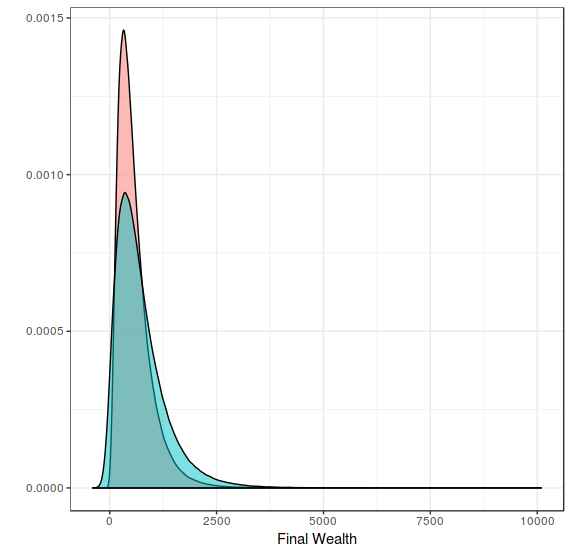
\includegraphics[scale=0.75]{./images/mort_final_wealth.png}
    \caption{Results of $1,000,000$ simulations for the both models with mortality. Final wealth obtained for every simulation. The blue one is the CPPI, and the red one is the Alternative. With $\pi = 0.5$, $\alpha = 0.343$, $\sigma = 0.1544$, $a = 10$, $T = 60$, $A = 0.5$ and $w = 1$.}
    \label{fig:mort_fw}
\end{figure}


Looking at Figure \ref{fig:mort_fw} we might note that the results are quite similar. Nevertheless, we can spot some differences in the shape of the non-central zones of the figure, where the Alternative Strategy seems to show less dispersion.

With a quick glimpse at Figure \ref{fig:mort_loss} we can already notice the great difference in the loss distribution of both schemes. It is clear that the CPPI is far more risky than the Alternative.

\begin{figure}[h]
    \centering
    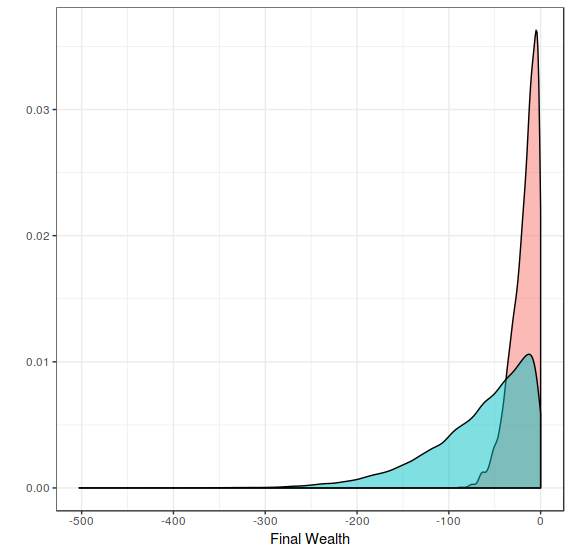
\includegraphics[scale=0.75]{./images/loss_both_mort.png}
    \caption{Results of $1,000,000$ simulations for the both models with mortality. Losses obtained for every simulation. The blue one is the CPPI, and the red one is the Alternative. With $\pi = 0.5$, $\alpha = 0.343$, $\sigma = 0.1544$, $a = 10$, $T = 60$, $A = 0.5$ and $w = 1$.}
    \label{fig:mort_loss}
\end{figure}

Since the conclusions extracted from just one value of $\pi$ may be misleading, let us iterate these simulations for many values of $\pi$ and $K$. In order to equalise the level of risk of the result of both strategies, we ought to make use of Formula \ref{eq:kes}, as we have done before. The problem is that we can not be sure that the assumptions and deduction from~\cite{a:guillen-optimisation} will be standing for this scenario that we are constructing. In fact, looking at the results of Figure~\ref{fig:es-es_mort_old} we can be sure that the measured Expected Shortfall are not the same for both strategies when in a Pooled Fund.

\begin{figure}[h]
    \centering
    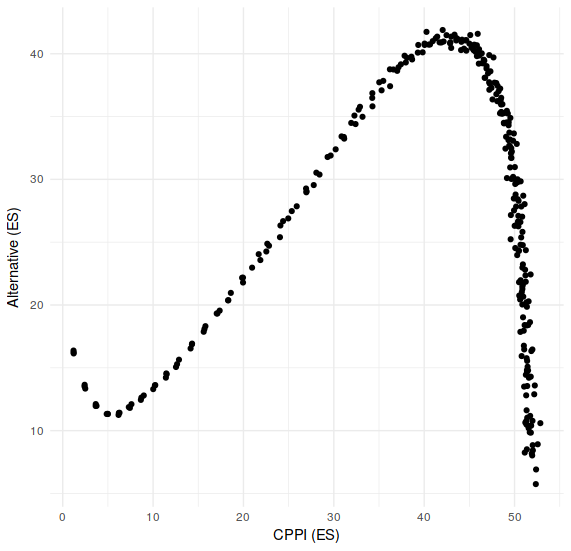
\includegraphics[scale=0.65]{./images/es-es.png}
    \caption{Expected Shortfall measured from the results of $100,000,000$ simulations for the both models with mortality, finding $K$ by using Formula~\ref{eq:kes}. With  many values for $\pi$, $A$ and $K$; $\alpha = 0.343$, $\sigma = 0.1544$, $a = 10$, $T = 60$ and $A = 0.5$ and $w = 1$.}
    \label{fig:es-es_mort_old}
\end{figure}

In order to pursue further results, the necessary value of $K$ in order to ensure more equal and accurate Expected Shortfall for both strategies has been found numerically, at the expense of more dispersion. These results are shown in Figure~\ref{fig:pi-a_mort}, Figure~\ref{fig:es-es_mort} and Table~\ref{tab:cppi_alt_mort}.


\begin{table}[h]
\centering
\caption{Results of $100,000$ simulations of both CPPI and Alternative models in a Pooled Fund, using different risk levels, with $\alpha = 0.343$, $\sigma = 0.1544$, $a = 10$, $T = 60$, $A = 0.5$ and $w = 1$.}
\label{tab:cppi_alt_mort}
\begin{tabular}{ccccccc}
\textbf{$\pi$} & \textbf{ES } & \textbf{$K$} & \textbf{CPPI ret} & \textbf{Alt ret} & \textbf{diff}  & \textbf{equiv $\pi$}\\
10  & 140.32  & 18.11 & 1.84 & 1.97 & 0.13 & 0.15 \\
20  & 88.75  & 88.41 & 2.13 & 2.79 & 0.65 & 0.34 \\
30  & 58.50  & 96.45 & 2.66 & 2.80 & 0.13 & 0.32 \\
40  & 20.85  & 165.75  & 3.13 & 3.59 & 0.46 & 0.49 \\
50  & -28.11 & 232.00  & 3.46 & 4.17 & 0.70 & 0.64 \\
60  & -73.18 & 294.04 & 3.83 & 4.67 & 0.83 & 1.06 \\
70  & -118.58 & 381.23 & 4.24 & 5.40 & 1.15 & 1.63 \\
80  & -153.69 & 424.03 & 4.77 & 5.85  & 1.07 & *                 \\
90  & -223.58 & 524.09 & 4.88 & 6.77 & 1.88 & *                 \\
100 & -261.12   & 618.38 & 5.16 & 6.79 & 1.62 & *

\end{tabular}
\end{table}


% The Pooled Fund has the effect of the wealth of all savers to increase dramatically. In fact, for lower risk levels as for $\pi < 0.5$, the final wealth of all simulations is so huge that the Expected Shortfall happenes to result positive and utterly large, instead of negative. So in order for the Alternative Strategy to equal that Expected Shortfall, the Formula \ref{eq:the_formula} leads to so hugely negative value of $K$ that the $\pi$ comes negative. Implying a short position in the market. Akwnoledging the non-sense that could derive from that decision, we have decided to cast out those simulations and simply state that this equivalence between the Expected Shortfall of both strategies is not valid for positive values of the Expected Shortfall.

As in the previous section, equivalent values of $\pi$ have been working as a succinct metric to compare the performance of this two strategies, taking into account both return and risk. Hence, as long as the equivalent $\pi$ remains above than the initial $\pi$, we can say that the Alternative Strategy is outperforming
the CPPI. Which is clear for most of the values of initial $\pi$ and a fixed value for $A$. Additionally, we can expand this results and find the iterated simulation of Table \ref{tab:cppi_alt_mort} for many values of $A$, as shown in Figure~\ref{fig:pi-a_mort}.

% \begin{figure}[h]
%     \centering
%     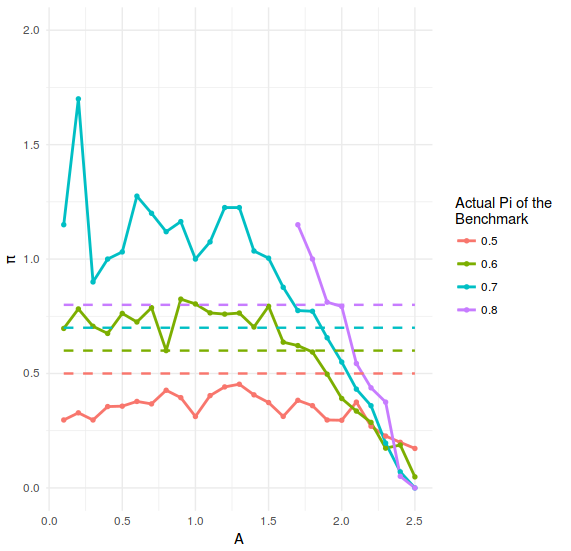
\includegraphics[scale=0.75]{./images/pi-A_mort_2.png}
%     \caption{Plot that shows the relation between equivalent $\pi$ and $A$, for many different initial $\pi$. From the results of $100,000$ simulations for each curve, with $\alpha = 0.343$, $\sigma = 0.1544$, $a = 10$, $T = 60$.}
%     \label{fig:pi-a_mort}
% \end{figure}

\begin{figure}
\centering
\begin{subfigure}{.5\textwidth}
    \centering
    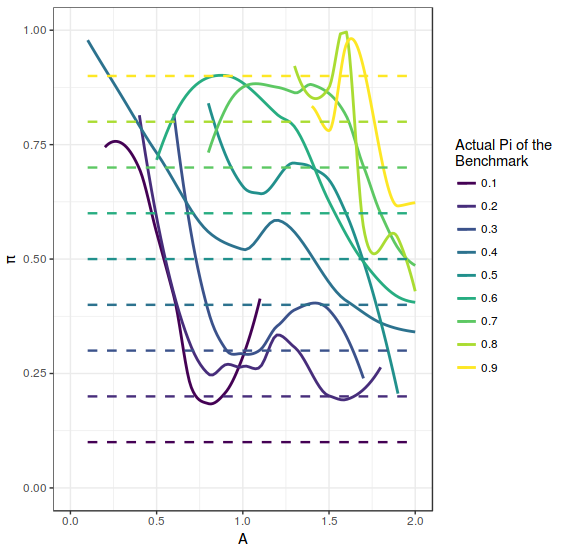
\includegraphics[scale=0.5]{./images/pi-a_mort2.png}
    \caption{Plot that shows the relation between equivalent $\pi$ and $A$.}
    \label{fig:pi-a_mort}
\end{subfigure}%
\begin{subfigure}{.5\textwidth}
    \centering
    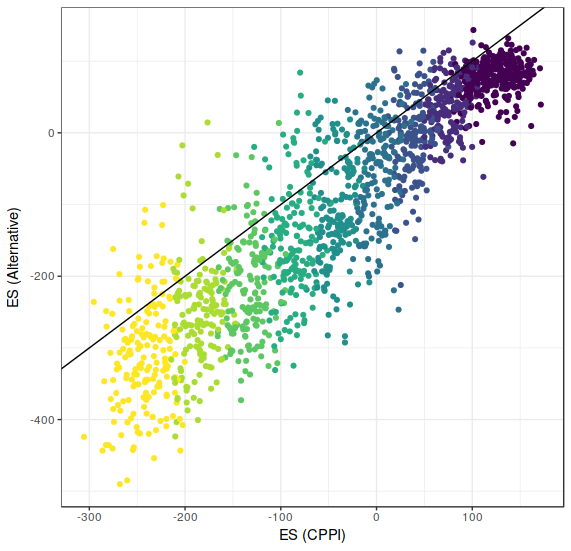
\includegraphics[scale=0.5]{./images/es-es_mort_new.png}
    \caption{Scatterplot that shows the equivalence between the Expected Shortfall derived from the simulations of Figure \ref{fig:pi-A_all-pis2}.}
    \label{fig:es-es_mort}
\end{subfigure}
\caption{Results from $20,000,000$ simulations performed for many different values of $\pi$ and $A$, with $\alpha = 0.343$, $\sigma = 0.1544$, $a = 10$, $T = 60$.}
\label{fig:compare_mort}
\end{figure}

The main difference we can note between Figure~\ref{fig:es-es_pi2} and Figure~\ref{fig:es-es_mort} is that the equivalence between Expected Shortfall tends also to be true, but is far more volatile in the case of a Pooled Fund. This leads to far more disperse result in Figure~\ref{fig:pi-a_mort} than in Figure~\ref{fig:pi-A_all-pis2}. Despite that, we can glimpse some patterns within the results that let us observe some distinctions between the results without and with mortality. Note that the values that are not present in the plot of Figure~\ref{fig:pi-a_mort} is because there were not value of equivalent $\pi$ for the CPPI capable of equaling the results of the Alternative. Note also that this happens more often for higher values of $\pi$.

Attending at the obtained results, we can see that outside of a Pooled Fund, the decision of whether the CPPI strategy or the Alternative is more worth it has to do with the value of $A$ alone, not with $\pi$. On the contrary, within the context of a Pooled Fund, we can see that the Alternative model shines over the CPPI for higher values of $\pi$. In fact, for higher values of $\pi$, the Alternative strategy outperforms the CPPI so much that often an equivalent value $\pi_b$ for the CPPI to equal the return of the Alternative simply does not exist. This result is of great importance, specially considiering that both strategies incur in the same risk level, as it is shown in Figure~\ref{fig:es-es_mort}.

As before, we can roughly observe a downhill behaviour of the plot.  This trend indicates that, for higher levels of $A$, where $A$ is interpreted as the inverse of the risk aversion, the Alternative strategy tends to be less relatively worth it, compared to the CPPI; even though in most cases the straight line stays above the dashed line over all values of $A$. Nonetheless, we can highlight a sweetspot around $A = 1.5$ where the plot gets to relative maximum for many levels of $\pi$.





\section{Tails Analysis}

At this point we should have notice that the real danger of investments does not resides solely within the standard concept of dispersion (standard deviation), nor within the ratio between return and dispersion. The true risk dwells in the worst case scenarios of the distributions, the tails. Where accumulated or great losses may strike down the whole investment plan. Hence, in order to address the risk analysis of any savings strategy, we need to take a closer look at the tails of their distributions. 


Taking a close look at Figure \ref{fig:both_fw}, we are not able to clearly state which one is \textit{less risky}. So far, we have been comparing the values of Expected Shortfall in order to get a sense of the risk. But, since the ES is actually just the average of the tail of the distribution, we will now discuss how we can pursue a more in-depth analysis for the distribution of those tails.

In this section, we will go one step further and try to fit some specific distribution to those tails. This way we will be able to see in more detail the behaviour of the losses of our strategies, and set more accurate risk measures.

\subsection{Definition of \textit{Tail}}

First things first. What is \emph{the} Tail of a distribution? The tail of a distribution is not a precisely defined term; it can have many different forms and definitions. Generally, the \textit{tail} is considered a broad term to name the extreme parts of a distribution. In other words, there is not some specific place where you stop being in the middle of the distribution and start being in the tail, and where to put that line is up to every case.

Let's say that we plot a distribution $Y$, the loss of a savings plan (note that negative losses imply profits). We decide to put the distinction between middle and tail at some point named $u$, so the tail would be everything that lands within $Y>u$.

If we understand the tail of a distribution as a distribution itself, we can move that tail to the origin and normalise its area. Thus, being positively defined as

\begin{align}
    Z = \qty(Y-u | Y>u)
\end{align}.

Once we have this definition, we can easily define the probability density as

\begin{align}
    F_Z(z)  &=  P(Z < z) = P\qty(Y-u < z | Y>u)  \\
            &=  P\qty(Y<z+u | Y>u) \\
            &= \frac{P\qty(Y<z+u, Y>u)}{P\qty(Y>u)}
\end{align}

And thus, deriving this expression we find that, for every $z>0$,

\begin{align}
    f_z(z) = \frac{f_y\qty(z+u)}{1-F_y(u)}\textit{.}
\end{align}

Interesting thing about this result, is that we can analytically relate the distribution of the tail $f_z(z)$ with the whole original distribution $f_y(z)$.

Therefore, we can say that, if the distribution of the losses obtained is $Y$, our tail could be defined as

\begin{align}
    F_u(y) = \qty( Y - u \leq y| Y > u ) \emph{.}
\end{align}

The Pickands-Balkema-de Haan theorem states that for a large class of distributions $X$, exists $u$ such as that $F_u$ is well approximated by the Generalized Pareto Distribution (GPD) $G$. Where the standard cumulative distribution function of the GPD can be defined as:


\[F_{\xi}(y) = \left\{
  \begin{array}{lr}
    1 - \qty(1 + \xi y)^{\sfrac{-1}{\xi}} & : \xi \neq 0\\
    1 - e^{-y} & : \xi = 0
  \end{array}
\right. \emph{.}
\]

Thus, we can seek that point $u$ from which our tail could fit a GPD. That would imply that, from that point $u$ forward, the distribution follows a GPD. The kind of GPD would be determined by the value of $\xi$. This number, usually called \emph{Extreme Value Index}, that determines  the shape of the distribution. The larger the value of $\xi$, the thicker the tail grows, and the slowly it converges to zero. In general:

\begin{itemize}
    \item $\xi > 0$. The tail does not converge to zero, ever. Power-law
    \item $\xi = 0$. The tail converges to zero at infinity. Exponential
    \item $\xi < 0$. The tail converges to zero in a finite point.
\end{itemize}

In what risk analysis concerns, the value of $\xi$ is crucial. Since we are studying the risk of a strategy looking at the tail of distributions where distribution are the frequency of losses, we could think that the wider or thicker the tail, the riskier the strategy. 

\subsection{Extreme Value Analysis: Fitting a General Pareto Distribution}

Let us repeat the simulation for the CPPI, using $\pi = 0.1$, and plot the histogram of its losses as an example.

\begin{figure}[H]
    \centering
    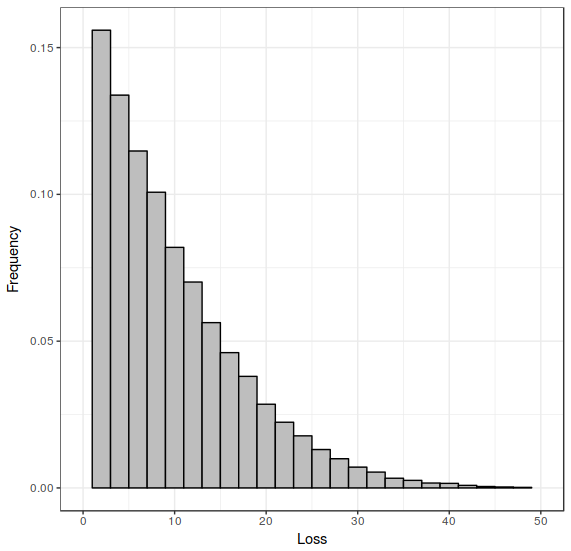
\includegraphics[scale=0.75]{images/cppi-losses-hist.png}
    \caption{Frequency Histogram of the losses of the CPPI strategy. Using $\pi = 0.1$, $\alpha = 0.0343$, $\sigma = 0.1544$ and $1000000$ simulations.}
    \label{fig:cppi-losses-histogram}
\end{figure}

If we now plot that density as points in a logarithmic scale, we might see something like the following:

\begin{figure}[H]
    \centering
    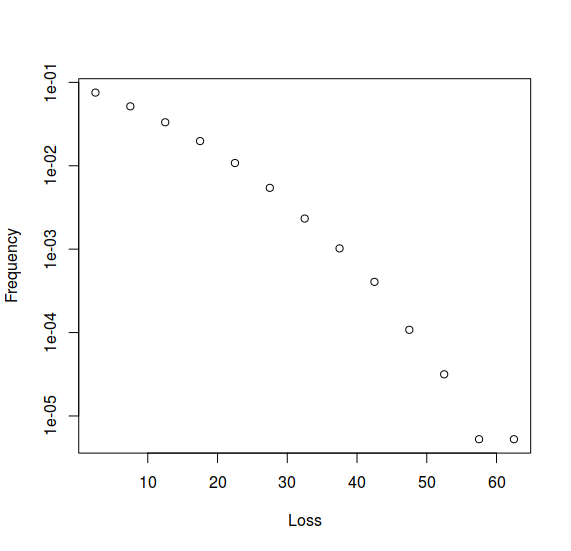
\includegraphics[scale=0.75]{images/cppi-dens-points.png}
    \caption{Density Distribution of the losses of the CPPI strategy in a logarithmic scale. Using $\pi = 0.1$, $\alpha = 0.0343$, $\sigma = 0.1544$ and $1000000$ simulations.}
    \label{fig:cppi-dens-points}
\end{figure}

Now, we could try to add here the Complementary Cumulative Distribution Function of a Generalized Pareto Distribution, and see if it fits to our distribution as it is now.

\begin{figure}[H]
    \centering
    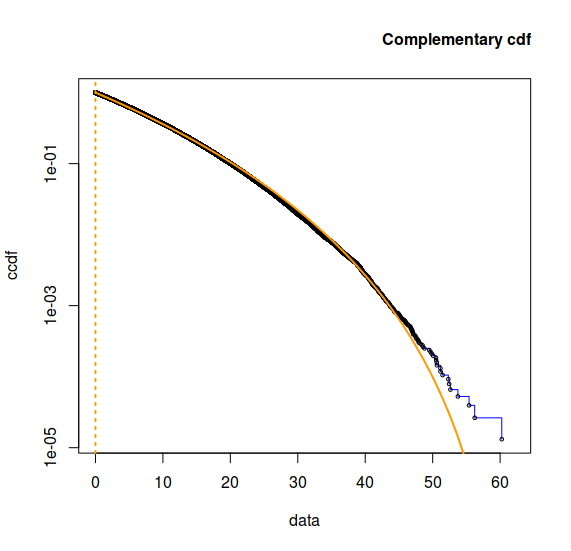
\includegraphics[scale=0.75]{images/cppi-ccdf-0.png}
    \caption{Density Distribution of the losses of the CPPI strategy in a logarithmic scale. Using $\pi = 0.1$, $\alpha = 0.0343$, $\sigma = 0.1544$ and $1000000$ simulations.}
    \label{fig:cppi-ccdf-0}
\end{figure}

Clearly, we can see how badly it fits for larger numbers. This indicates that our distribution is not following a GPD. Nevertheless, we can still find a proper $u$ for which it would.




\subsection{Convergence of the Expected Shortfall}

So far, we have addressed the necessity of studying the tail of loss danger using the Expected Shortfall. It is quite straightforward and it easily assesses the risk of the tail. But since it is nothing more than a simple mean, it can arise some issues. 

We talked about how the tail of a distribution can be considered a distribution by itself. Thus, the mean of the tail intends to be a summary statistic of this distribution. Despite that, we know that the arithmetic mean is not always a good summary statistic for every given distribution. There are some distributions from which the mean is not the best suited statistic to get a reliable feel of its \emph{general tendency}, especially on very skewed distributions.

Moreover, without previous knowledge about the distribution we may encounter, it exists the possibility of facing a distribution whose arithmetic mean does not exist. This possibility arises a very disturbing problem: The computed value of the Expected Shortfall should not exist. Since we are working with simulated data, and thus finite numbers, we will never face an infinite arithmetic mean. This implies that in order to ensure the reliability of the Expected Shortfall, we first need to check whether its computation makes sense or not.

In Figure \ref{fig:loss_both} we see the density curve of the loss tails of both methods. If we compute the histogram and set the bars of the histogram as points, we can build a scatterplot. 
In Figure \ref{fig:lm-tails} we can see this scatter plot of their logarithmic density points. It is of great interest noticing that, whereas both tails follow a linear model quite accurately (after taking logarithms), the \textit{Alternative} scheme has a much sharper descending trend. Which would mean that its \textit{Expected Shortfall} is far less likely to be infinite in any analytical distribution. This suggests us that the computed value of the Expected Shortfall is much more reliable for the \textit{Alternative} scheme than for the CPPI one.

\begin{figure}[h]
    \centering
    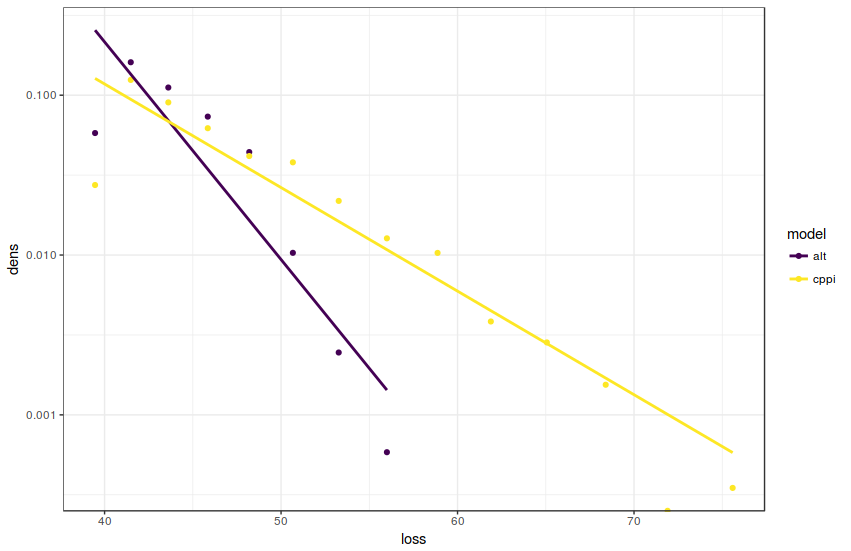
\includegraphics[scale=0.5]{images/lm_tails.png}
    \caption{Scatter plot and linear regression of the logarithm of the density points of the \textit{CPPI} and \textit{Alternative} methods.}
    \label{fig:lm-tails}
\end{figure}


\section{Conclusions}

As a result of this work we have given a bit of context and explanation to standard risk measures and utilised them to revise and expand the results obtained from \cite{a:guillen-optimisation}. It has been shown that for more values for $\pi$ and $A$ the same conclusions can be extracted: If a saver is capable of assuming up to $K$ losses, then the optimal strategy is to invest $A$ times the accumulated wealth in risky assets, where $A$ is defined as the inverse of the risk aversion.

Additionally, following the logic provided by the comparison of the benchmark and the proposed strategy, the same analysis has been applied within the context of a Pooled Fund, that takes into account mortality. First, the purpose has been to present and simulate the results obtained of utilising such scheme, and we have seen that the computed returns presented in Table~\ref{tab:cppi_alt_mort} corresponding to the Pooled Fund are considerably higher than the presented in Table~\ref{tab:cppi_alt} corresponding to the simpler approach. These results highlight the potential profits that the industry could gain from using such schemes in Pension Plans, and the necessary academic interest in studying them.

Then, we aimed to test whether the same conclusions and insights gotten from~\cite{a:guillen-optimisation} can be extrapolated when adding Mortality and a Pooled Fund. The results presented in Figure~\ref{fig:es-es_mort_old} indicates that whereas some of the assumptions considered in~\cite{a:guillen-optimisation} in order to develop Equation~\ref{eq:kes} are clearly correct (see Figure~\ref{fig:es-es_pi2}), they might not be holding true anymore within the context of Pooled Funds. Additionally, results presented in Figure~\ref{fig:pi-a_mort} have shown us that there the same conclusion can be extracted without and within Pooled Funds: If a saver is capable of assuming up to $K$ losses, then the optimal strategy is to invest $A$ times the accumulated wealth in risky assets, where $A$ is defined as the inverse of the risk aversion. This stands of even greater importance for values of $A$ closer to $1.5$. And, in many cases, the performance of the alternative strategy dwarfs the returns obtained by the CPPI, as much as concluding that there is no achievable level of risk that lets the CPPI equal the higher results obtained by the alternative strategy.

Moreover, we have added to these previous analysis the usage of a new kind of risk measure based on the Extreme Value Analysis of the tails of the obtained distributions, providing a location and scale free risk measure, especially in situations where location-dependent measures are less reliable. The purpose has been to highlight the main differences and limitations of different risk measures and stress the necessity of adding location and scale free risk measures, as the Extreme Value Index, to the standard toolkit of risk analysis when optimising financial investments and savings strategies. When applied to the strategies of interest, we have been able to spot some interesting insights, as the decrease of the thickness of the tails obtained by the strategies where the Alternative Scheme is used. Indicating that even for the same values of Expected Shortfall, we can find that one strategy shows less risk than the other, helping the investor or institution contrast the risk level of different strategies.

An immediate consequence of adding mortality to the scheme of any strategy is that the investor the survives the long run manages to largely increase their wealth. This shrinkes the risk of losses dramatically. This kind of risk has to be necessarily different in nature from the risk just derived from the dispersion of the expected return. From the results extracted from Figure~\ref{fig:evi-es} we might deduce that this condition is fairly better reflected by the Extreme Value Index rather than the Expected Shortfall, proving that the EVI can function as a location and scale free risk measure.

We conclude that extreme caution ought to be taken when making conclusions out of apparently less risky scenarios; and that a Location and Scale free risk measure could give more insight in such situations. Furthermore, pension plans providers could benefit greatly from using of both the Alternative Model and the context of Pooled Funds, separated or together, for most risk profiles. With the added simplicity of using maximum allowed loss $K$ as a metric for settling the risk profile of savers, instead of more abstract ones as "risk aversion".

Further research could be of extreme interest on the Pooled Fund scheme. The structure presented in this work is utterly simplistic and could be extended. Major improvements could reside in studying more levels for the percentage returned to the pool, when an investor dies (in this work we have always considered a $100\%$, even acknowledging that that could be unrealistic) or adding age variability to the simulated investors.


\begin{appendices}
\section{Simple CPPI Code}\label{ap:cppi-simple}


\begin{lstlisting}[language = R]
nsim <- 10000

pi <- 0.1
alpha <- 0.0343 # Expected return of the risky market
sigma <- 0.1544 # Expected volatility of the risky market
a <- 10 # Factor 'a'
years <- 60 # Total time

C <- append(rep(a, round(years/2)),rep(-a, round(years/2)))

X_T <- c()

for (j in 1:nsim){
	x <- c()
	x[1] <- a # Initial wealth

	for (i in 1:(years-1)){
		random <- rnorm(1, mean = alpha, sd = sigma)
		x[i+1] <- x[i]*(1+random)*pi + (1-pi)*x[i] + C[i+1]
	}
	X_T[j] <- x[years]

}
\end{lstlisting}


\section{Simple Alternative Code}\label{ap:alt-simple}

\begin{lstlisting}[language = R]

# Computation of 'pi' value function
fpi <- function(A, K, X, C, time){
	g <- sum(C[-c(1:time)])
	xpi <- A*(K + X + g)
	return(xpi)
}

nsim <- 10000

pi <- 0.1
alpha <- 0.0343 # Expected return of the risky market
sigma <- 0.1544 # Expected volatility of the risky market
a <- 10 # Factor 'a'
years <- 60 # Total time

C <- append(rep(a, round(years/2)),rep(-a, round(years/2)))

X_T <- c()

for (j in 1:nsim){
	x <- c()
	x[1] <- a # Initial wealth

	for (i in 1:(years-1)){
		random <- rnorm(1, mean = alpha, sd = sigma)
		pi <- fpi(A,K,X,C,i)
		x[i+1] <- x[i]*(1+random)*pi + (1-pi)*x[i] + C[i+1]
	}
	X_T[j] <- x[years]

}
\end{lstlisting}

\section{Mortality Code}\label{ap:mort-code}

\begin{lstlisting}[language = R]

# Computation of 'pi' value function
fpi <- function(A, K, X, C, time){
	g <- sum(C[-c(1:time)])
	xpi <- A*(K + X + g)
	return(xpi)
}

  ### CPPI ###

	C <- append(rep(a, round(years/2)),rep(-a, round(years/2)))
	mort_table <- fread("mortality.csv")/1000
	X_T <- c()

	for (j in 1:nsim){
		x <- c()
		x[1] <- a # Initial wealth
		number_humans_alive <- starting_humans

		for (i in 1:(years-1)){
			prob_mort <- mort_table$total[i+starting_age-1]
			number_deads <- rbinom(1,number_humans_alive,prob_mort)
			number_humans_alive <- number_humans_alive - number_deads


			random <- rnorm(1, mean = alpha, sd = sigma)
			x[i+1] <- x[i]*(1+random)*pi + (1-pi)*x[i] + C[i+1] + (x[i]*number_deads/number_humans_alive)*w
		}
		X_T[j] <- x[years]
  }

  ### Alternative ###

	C <- append(rep(a, round(years/2)),rep(-a, round(years/2)))
	mort_table <- fread("mortality.csv")/1000
	X_T <- c()

	for (j in 1:nsim){
		x <- c()
		x[1] <- a # Initial wealth
		number_humans_alive <- starting_humans

		for (i in 1:(years-1)){
			prob_mort <- mort_table$total[i+starting_age-1]
			number_deads <- rbinom(1,number_humans_alive,prob_mort)
			number_humans_alive <- number_humans_alive - number_deads

      pi <- fpi(A,K,X,C,i)
			random <- rnorm(1, mean = alpha, sd = sigma)
			x[i+1] <- x[i]*(1+random)*pi + (1-pi)*x[i] + C[i+1] + (x[i]*number_deads/number_humans_alive)*w
		}
		X_T[j] <- x[years]
	}
\end{lstlisting}

\end{appendices}{}

%-----------------------------------------------------------------
%	BIBLIOGRAPHY
%-----------------------------------------------------------------


\printbibliography[heading=bibintoc]
\setcounter{secnumdepth}{0}
% \section{References}
% \printbibliography[title={Articles}, type=article, heading=subbibliography]
% \printbibliography[title={Books}, type=book, heading=subbibliography]
% \printbibliography[title={Websites}, type=online , heading=subbibliography]
% \printbibliography[title={Basic}, keyword=basic , heading=subbibliography]
% \printbibliography[title={Data Sets}, keyword=dataset , heading=subbibliography]
% \printbibliography[title={Licenses}, keyword=license , heading=subbibliography]
\end{document}
